\documentclass{article}


\usepackage[T1]{fontenc}

\usepackage{polski}
\usepackage[utf8]{inputenc}
\usepackage[polish]{babel}

\usepackage{graphicx}
\usepackage{amsmath}

\usepackage{psfrag}
\begin{document}

\pagestyle{empty}
\psfrag{\{EMPTY TITLE\}}{
	$ $
}
\psfrag{\{X LABEL\}}{
	\begin{picture}(0,0)
	\put(-95, -5){Liczba wierzchołków w grafie $G$ ($\left| E \right| = \frac{1}{10} \cdot \binom{\left| V \right|}{2}$)}
	\end{picture}
}
\psfrag{\{Y LABEL\}}{
	\begin{picture}(0,0)
	\put(-30, 10){Wartość rozwiązania}
	\end{picture}
}

\psfrag{WARTOSCROZWIAZANIA}{\scriptsize wartość rozwiązania}
\psfrag{NAJLEPSZEROZWIAZANIE}{\scriptsize najlepsze rozwiązanie}
\psfrag{DOLNEOSZACOWANIE}{\scriptsize dolne ograniczenie}

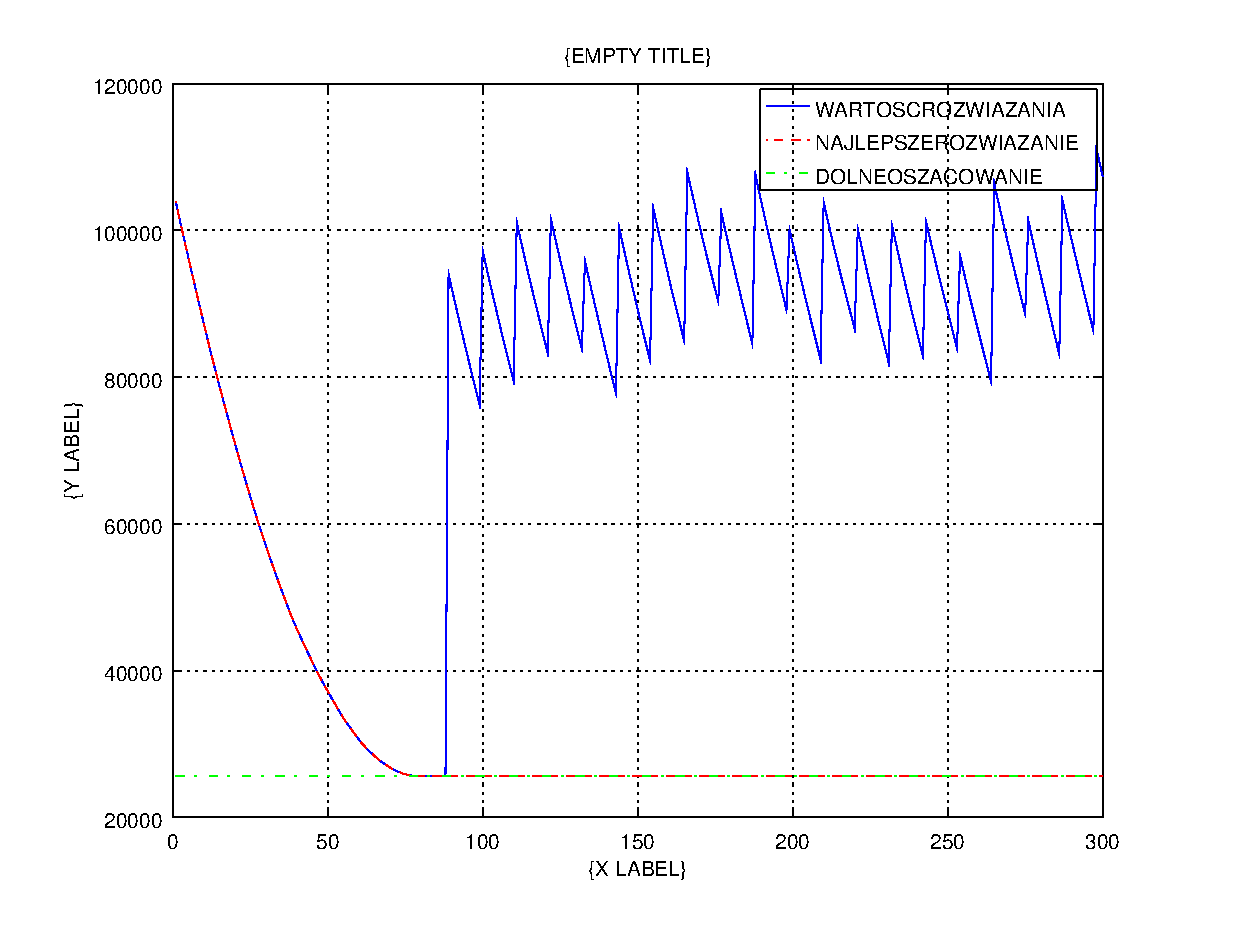
\includegraphics[width=\textwidth]{out}
\end{document}